In previous chapter we introduced the notions of membrane and membrane structure.

% Place objects in the regions.

The next step is to place certain objects in the regions delimited by the membranes. The objects are identified by their names, mathematically symbols from a given alphabet.

% Multisets of objects.

Several copies of the same object can appear in a region, so we will work with multisets of objects.

% Evolution rules

In order to obtain a computing device, we will allow the objects to evolve according to evolution rules. Any object, alone or together with another objects, can be transformed in other objects, can pass through a membrane, and can dissolve the membrane in which it is placed.

% Parallelism

All objects evolve at the same time, in parallel manner across all membranes.

% Priorities

The evolution rules are hierarchized by a priority relation, which is a partial order.

% P system

These aspects all together forms a P system as introduced in \cite{Paun98}. An example of a P system containing rules for computing the Fibonacci sequence can be seen in the figure \ref{fig:p_system_fibonacci}.


In section~\ref{sec:definitions} we will provide formal definition of a P system.

\section{Definitions} % (fold)
\label{sec:definitions}

% Definition taken from my article

Let $\Sigma$ be a set of objects. Recall that $\mathbb N^\Sigma$ contains all multisets of objects from $\Sigma$. {\bf Membrane configuration} is a tuple $(T, l, c)$, where:
\begin{itemize}
  \item $T$ is a rooted tree,
  \item $l\in\mathbb N^{V(T)}$ is a mapping that assigns for each node of $T$ a number (label), where $l(r_T)=1$, so the skin membrane is always labeled with 1,
  \item $c\in(\mathbb N^\Sigma)^{V(T)}$ is a mapping that assigns for each node of $T$ a multiset of objects from $\Sigma$, so it represents the contents of the membrane.
\end{itemize}

{\bf Active P system} is a tuple $(\Sigma, C_0, R_1, R_2, \dots , R_m)$, where:
\begin{itemize}
  \item $\Sigma$ is a set of objects,
  \item $C_0$ is initial membrane configuration,
  \item $R_1,R_2,\dots R_m$ are finite sets of rewriting rules associated with the labels $1,2,\dots,m$ and can be of forms:
  \begin{itemize}
    \item $u\rightarrow w$, where $u\in \Sigma^+$, $w\in (\Sigma\times\{\cdot, \uparrow, \downarrow_j\})^*$ and $1\leq j\leq m$,
    \item $u\rightarrow w\delta$, where $u\in \Sigma^+$, $w\in (\Sigma\times\{\cdot, \uparrow, \downarrow_j\})^*$ and $1\leq j\leq m$,
    \item $u\rightarrow [_j v]_j$, where $u\in \Sigma^+, v\in \Sigma^*$ and $1\leq j\leq m$.
  \end{itemize}
\end{itemize}

Although rewriting rules are defined as strings, $u,v$ and $w$ represent multisets of objects from $\Sigma$. For the first two forms, each rewriting rule may specify for each objects on the right side, whether it stays in the current region (we will omit the symbol $\cdot$), moves through the membrane to the parent region ($\uparrow$)
or to a specific child region ($\downarrow_j$, where $j$ is a label of a membrane).
We denote these transfers with an arrow immediately after the symbol.
An example of such rule is the following: $abb\rightarrow ab\downarrow_2 c\uparrow c$.
Symbol $\delta$ at the end of the rule means that after the application of the rule, the membrane is dissolved and its contents (objects, child membranes) are propagated to the parent membrane.
Active P systems differs from classical (passive) P systems in ability to create new membranes by rules of the third form.

% applicable rule definition

For active P system $(\Sigma, C_0, R_1, R_2, \dots , R_m)$, configuration $C = (T, l, c)$, membrane $d\in V(T)$ with label $j = l(d)$ the rule $r\in R_j$ is {\bf applicable} iff:
\begin{itemize}
  \item $r = u\rightarrow w$ and $u\subseteq c(d)$ and $\forall (a,\downarrow_k)\in w \exists d_2\in V(T): l(d_2)=k \wedge parent(d_2) = d$,
  \item $r = u\rightarrow w\delta$ and $u\subseteq c(d)$ and $\forall (a,\downarrow_k)\in w \exists d_2\in V(T): l(d_2)=k \wedge parent(d_2) = d$ and $d\neq r_T$,
  \item $r = u\rightarrow [_k v]_k$ and $u\subseteq c(d)$.
\end{itemize}

% TODO result of the rule application

For the simplicity of proofs it is convenient to introduce a variant with a global limit upon the membrane structure. We achieve this by restricting the rule application such that if the rule would result in a structure exceeding the limit, the rule will not be applicable.

{\bf Active P system with a limit on total number of membranes} is a tuple $(\Sigma, L, C_0, R_1, R_2, \dots , R_m)$, where $(\Sigma, C_0, R_1, R_2, \dots , R_m)$ is an active P system and $L\in \mathbb N$ is a limit on total number of membranes. Anytime during the computation, a confuguration $(T, l, c)$ is not allowed to have more than $L$ membranes, so the following invariant holds: $|V(T)|\leq L$.

This is achieved by adding a constraint for rule of the form $r = u\rightarrow [_k v]_k$, which is defined to be applicable iff $u\subseteq c(d)$ and $|V(T)|<L$. If the number of membranes is equal to $L$, there is no space for newly created membrane, so in that case such rule is not applicable.

A {\bf computation step} of P system is a relation $\Rightarrow$ on the set of configurations such that $C_1 \Rightarrow C_2$ holds iff there is an applicable rule in a membrane in $C_1$ such that applying that rule would result in $C_2$.

An {\bf infinite computation} of a P system is an infinite sequence of configurations $\{C_i\}_{i=0}^\infty$, where $\forall i: C_i\Rightarrow C_{i+1}$.

A {\bf finite computation} of a P system is a finite sequence of configurations $\{C_i\}_{i=0}^n$, where $\forall i: C_i\Rightarrow C_{i+1}$.

A {\bf halting computation} of a P systems is a finite computation $\{C_i\}_{i=0}^n$, where there is no applicable rule in the last configuration $C_n$.

% Result of a computation

There are two possible ways of assigning a result of a computation:

\begin{enumerate}
    \item By considering the multiplicity of objects present in a designated membrane in a halting configuration. In this case we obtain a vector of natural numbers. We can also represent this vector as a multiset of objects or as Parikh image of a language.
    \item By concatenating the symbols which leave the system, in the order they are sent out of the skin membrane (if several symbols are expelled at the same time, then any ordering of them is considered). In this case we generate a language.
\end{enumerate}

The result of a single computation is clearly only one multiset or a string, but for one initial configuration there can be multiple possible computations. It follows from the fact that there can be more than one applicable rule in each configuration.

Each rewriting rule may specify for each symbol on the right side, whether it stays in the current region, moves through the membrane to the parent region or through membrane to one of the child regions. An example of such rule is the following: $abb\rightarrow (a,here)(b,in)(c,out)(c,here)$.

% Configuration

% !TEX root = ../diz.tex
A {\em configuration} of a P system is represented by its membrane structure and the multisets of objects in the regions.

% Step

A {\bf computation step} of P system is a relation $\Rightarrow$ on the set of configurations such that $C_1 \Rightarrow C_2$ iff:

For every region in $C_1$ (suppose it contains a multiset of objects $w$) the corresponding multiset in $C_2$ is the result of applying a multiset of maximal simultaneously applicable multiset rewriting rules in $R^{msap}_w$ to $w$.

In other words, a maximal multiset of rules is applied in each region.

For example, let's have two regions with multisets $aa$ and $b$. In the first region there is a rule $a\rightarrow b$ and in the second membrane there is a rule $b\rightarrow aa$. The only possible result of a computation step is $bb$, $aa$. The first rule was applied twice and the second rule once. No more object could be consumed by rewriting rules.

% Computation

% !TEX root = ../diz.tex
{\bf Computation} of a P system consists of a sequence of steps. The step $S_i$ is applied to result of previous step $S_{i-1}$. So when $S_i = (C_j,C_{j+1})$, $S_{i-1} = (C_{j-1},C_j)$.

% Result of a computation

There are two possible ways of assigning a result of a computation:

\begin{enumerate}
    \item By considering the multiplicity of objects present in a designated membrane in a halting configuration. In this case we obtain a vector of natural numbers. We can also represent this vector as a multiset of objects or as Parikh image of a language.
    \item By concatenating the symbols which leave the system, in the order they are sent out of the skin membrane (if several symbols are expelled at the same time, then any ordering of them is accepted). In this case we generate a language.
\end{enumerate}

The result of a computation is clearly only one multiset or a string, but for one initial configuration there can be multiple possible computations. It follows from the fact that there exist more than one maximal multiset of rules that can be applied in each step.

\begin{figure}[h]
  \centering
  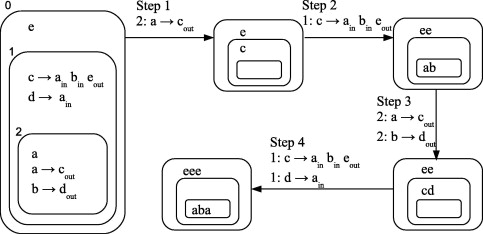
\includegraphics[width=0.8\textwidth]{img/p_system_fibonacci.jpg}
  \caption{P system computing a Fibonacci sequence \cite{Buiu201233PSystemFibonacci}}
  \label{fig:p_system_fibonacci}
\end{figure}

% TODO: quality vs quantity aspects.


% section definitions (end)

\section{P system variants} % (fold)
\label{sec:p_system_variants}
% !TEX root = ../diz.tex
Besozzi in his PhD thesis (see \cite{Besozzi:PhD:2004}) formulates three criteria that a good P system variant should satisfy:

\begin{enumerate}
	\item It should be as much realistic as possible from the biological point of view, in order not to widen the distance between the inspiring cellular reality and the idealized theory.
	\item It should result in computational completeness and efficiency, which would mean to obtain universal (and hence, programmable) computing devices, with a powerful and useful intrinsic parallelism;
	\item It should present mathematical minimality and elegance, to the aim of proposing an alternative framework for the analysis of computational models.
\end{enumerate}

In membrane computing, many models are equal in power with Turing machines. We should say they are Turing complete (or computationally complete), but because the proofs are always constructive, starting the constructions from these proofs from universal Turing machines or from equivalent devices, we obtain universal P systems (able
to simulate any other P system of the given type). That is why we speak about universality results, and not about computational completeness.

\subsection{Accepting vs generating} % (fold)
\label{sub:accepting_vs_generating}

In the Chomsky hierarchy, there are language acceptors (finite automata, Turing machines) and language generators (formal grammars).

% Accepting grammars

Bordhin in \cite{Bordihn99acceptingpure} extends grammars to allow for accepting languages by interchanging the left side with the right side of a rule. The mode will apply rewriting rules to an input word and accept it when it reaches the starting nonterminal. However, the input word consists of terminal symbols, which could not be rewritten when using original definition, hence they consider the pure version of various grammar types where they give up the distinction between terminal and nonterminal symbols.

% Accepting vs generating common results

The regular, context-free, context-sensitive and recursively enumerable languages were shown to have equal power in accepting and generating mode.
Some other grammars (programmed grammars with appearance checking) are shown to be more powerful in accepting mode than in generating mode.
For deterministic Lindenmayer systems, the generating and accepting mode are incomparable.

% Accepting vs generating P system results

It can be interesting to investigate accepting and generating mode also in P system variants. Barbuti in \cite{Barbuti:2010:AcceptingGenerating} shown that in the nondeterministic case, when either promoters or cooperative rules are allowed, acceptor P systems have shown to be universal. The same in known to hold for the corresponding classes of nondeterministic generator P systems. In the deterministic case, acceptor P systems have been shown to be universal only if cooperative rules are allowed. Universality has been shown not to hold for the corresponding classes of generator P systems.

% subsection accepting_vs_generating (end)

\subsection{Active vs passive membranes} % (fold)
\label{sub:active_vs_passive_membranes}

% TODO: need citations
Most of the studied P system variants assumes that the number of membranes can only decrease during a computation, by dissolving membranes as a result of applying evolution rules to the objects present in the system.
A natural possibility is to let the number of membranes also to increase during a computation, for instance, by division, as it is well-known in biology. Actually, the membranes from biochemistry are not at all passive, like those in the models briefly described above.
For example, the passing of a chemical compound through a membrane is often done by a direct interaction with the membrane itself (with the so-called protein channels or protein gates present in the membrane); during this interaction, the chemical compound which passes through membrane can be modified, while the membrane itself can in this way be modified (at least locally).

In \cite{Paun99ActiveMembranes} P\u{a}un considers P systems with active membranes where the central role in the computation is played by the membranes: evolution rules are associated both with objects and membranes, while the communication through membranes is performed with the direct participation of the membranes; moreover, the membranes can not only be dissolved, but they also can multiply by division. An elementary membrane can be divided by means of an interaction with an object from that membrane.

% Polarization

Each membrane is supposed to have an electrical polarization (we will say charge), one of the three possible: positive, negative, or neutral. If in a membrane we have two immediately lower membranes of opposite polarizations, one positive and one negative, then that membrane can also divide in such a way that the two membranes of opposite charge are separated; all membranes of neutral charge and all objects are duplicated and a copy of each of them is introduced in each of the two new membranes.
The skin is never divided.
If at the same time a membrane is divided and there are objects in this membrane which are being rewritten in the same step, then in the new copies of the membrane the result of the evolution is included.

In this way, the number of membranes can grow, even exponentially. As expected, by making use of this increased parallelism we can compute faster.
For example, the SAT problem, which is NP complete, can be solved in linear time, when we consider the steps of computation as the time units.
Moreover, the model is shown to be computationally universal.

% subsection active_vs_passive_membranes (end)

\subsection{Context in rules} % (fold)
\label{sub:context_in_rules}

% Cooperative / Non-cooperative

Rewriting rules in P systems can be cooperative and non-cooperative, like in Chomsky's context-free and context-sensitive grammars. Non-cooperative rules are restricted to use only one object on the left side and cooperative rules do not have this restriction.
P systems with cooperative rules are universal \cite{Paun98}, while P systems with non-cooperative rules only characterize Parikh image of context-free languages ($PsCF$) \cite{Sburlan05dragos}.

% Catalytic P systems

P\u{a}un \cite{Paun98} also defines P systems with catalysts where catalysts are a specified subset of the alphabet. Rewriting rules can contain catalysts, which are not modified by applying the rule. Surprisingly, P systems with catalytic rules are universal, actually two membranes in the P system are sufficient to achieve universality.

In systems where only catalytic rules (purely catalytic systems \cite{Ibarra:03:Catalytic}), three catalysts are enough \cite{Freund2005TwoCatalysts}.

% Two catalysts

Freund in \cite{Freund2005TwoCatalysts} also shows that two catalysts and one membrane are enough and raised an open problem whether one catalyst is sufficient. He conjectured that for computationally universal P systems the results obtained in this paper are optimal not only with respect to the number of membranes (2), but also with respect to the number of catalysts.

% Catalysts are too powerful

From some point of view, catalysts are way too powerful in restricting the parallelism - they directly participate in the rules, hence the number of catalytic rules that can be applied in one step, is bounded by number of catalysts.

A variant with promoters and inhibitors have been proposed (see \cite{Ionescu:jucs_10_5:on_p_systems_with}).

% Promoters

In the case of promoters, the rules are possible only in the presence of certain symbols. An object $p$ is a promoter for a rule $u\rightarrow v$ and we denote this by $u\rightarrow v|_{p}$, if the rule is active only in the presence of object $p$. Note that unlike in the case with catalysts, promoters allow the associated rules to be applied as many times as possible.

% Inhibitors

An object $i$ is inhibitor for a rule $u\rightarrow v$ and we denote this by $u\rightarrow v|_{\neg i}$, if the rule is active only if inhibitor $i$ is not present in the region.
One of our results (see section \ref{sec:inhibitors}) uses inhibitors as a tool to achieve universality for sequential P systems.


% One catalyst with promoters / inhibitors

Ionescu in \cite{Ionescu:jucs_10_5:on_p_systems_with} shows that P systems with non-cooperative catalytic rules with only one catalyst and with promoters / inhibitors are universal.

% Zero catalysts with inhibitors

Non-cooperative rules with no catalysts and with inhibitors were studied in \cite{Sburlan:2006:FurtherResultsPromotersInhibitors}, the equivalence with Lindenmayer systems ($ET0L$ as defined in section \ref{sec:lindenmayer_systems}) was proved.

% Simple cooperative system

Dang \cite{Ibarra04dang} proposes a simple cooperative system ($SCO$) as a P system where the only rules allowed are of the form $a\rightarrow v$ or of the form $aa\rightarrow v$, where $a$ is a symbol and $v$ is a (possibly null) string of symbols not containing $a$. This variant is investigated with various modes of parallelism, so their results will be mentioned in the subsection \ref{sub:parallelism_options}

% subsection context_in_rules (end)

\subsection{Rules with priorities} % (fold)
\label{sub:rules_with_priorities}

In the original definition of a P system \cite{Paun98}, a partial order relation over set of rewriting rules have been specified. The rule can be used only if no rule of a higher priority in the region can be applied at the same time.

Sos\'ik in \cite{Sosik:2002:WithoutPriorities} showed that the priorities may be omitted from the model without loss of computational power.

% subsection rules_with_priorities (end)

\subsection{Energy in P systems} % (fold)
\label{sub:energy_in_p_systems}

Various notions of energy has been proposed for use in P systems. P\u{a}un in \cite{Paun:2001:Energy} considers a P system where each evolution rule ``produces'' or ``consumes'' some quantity of energy, in amounts which are expressed as integer numbers. In each moment and in each membrane the total energy involved in an evolution step should be positive, but if ``Too much'' energy is present in a membrane, then the membrane will be destroyed (dissolved). This variant was investigated in two cases, both were shown to be universal:

\begin{enumerate}
	\item when using only two membranes and unbounded amount of energy,
	\item when using arbitrarily many membranes and a bounded energy associated with rules
\end{enumerate}

Freund in \cite{Freund:2004:SequentialEnergy} introduced a new variant where the rules are assigned directly to membranes (every rule consume objects on one side of the membrane and produce objects on the other side) and every membrane carries an energy value that can be changed during a computation by objects passing through the membrane.

This variant is universal even in sequential mode if we allow priorities on the objects. When omitting the priority relation, only the family of Parikh sets generated by context-free matrix grammars ($PsMAT$ as defined in section \ref{sec:matrix_grammars}) is obtained.

% subsection energy_in_p_systems (end)

\subsection{Symport / antiport rules} % (fold)
\label{sub:symport_antiport_rules}

P\u{a}un in \cite{Paun:2002:SymportAntiport} proposes a new way of communicating between membranes.

Symports allow two chemicals to pass together through a membrane in the same direction using symport rules of type $(ab,in)$ or $(ab,out)$.
Antiports allow two chemicals to pass simultaneously through a membrane in opposite directions using antiport rules of type $(a,in;b,out)$.

Surprisingly, a P system variant, where only the symport / antiport rules are used are computationally complete. Five membranes are enough for this result. If more than two chemicals may collaborate when passing through membranes, two membranes are sufficient for universality. These results are proven in \cite{Paun:2002:SymportAntiport}.

% subsection symport_antiport_rules (end)

\subsection{Parallelism options} % (fold)
\label{sub:parallelism_options}

Original definition of P system (see \cite{Paun98}) uses maximal parallelism when doing a step of computation. There is an obvious biological motivation relying on the assumption that ``if we wait long enough, then all reaction which may take place will take place''. This condition is rather powerful, because it decreases the non-determinism of the system's evolution. For various reasons ranging from looking for more realistic models to just the mathematical challenge, the maximal parallelism was questioned.

% Sequential mode

Dang in \cite{Dang04Sequential} investigates the sequential mode. In each step, from the set of applicable rules across all membrane one is nondeterministically chosen and applied.

\begin{definition}
  \label{def:computation_step_of_a_sequential_P_system}
  A {\bf computation step of a sequential P system} is a relation $\Rightarrow$ on the set of configurations such that $C_1 \Rightarrow C_2$ holds iff there is an applicable rule in a membrane in $C_1$ such that applying that rule can result in $C_2$.
\end{definition}

For purely catalytic systems with 1 membrane, the sequential mode generates only the semilinear sets and thus is strictly weaker than the maximally parallel version.
Sequential version of symport / antiport systems are equivalent to vector addition systems making it strictly weaker than the original maximally parallel version.

Investigation of the sequential mode continues in \cite{Ibarra05Active}. Sequential P system without priorities with cooperative rules with rules for membrane dissolution are not universal by showing they can be simulated by vector addition systems with states (VASS).
This holds even when the membrane creation is allowed for bounded number of created membranes. However, if any number of membranes are allowed to be created, the system becomes universal. This result was shown by simulation of the register machine (see section \ref{sec:register_machines}).

We have further investigated this variant (sequential P system without priorities with cooperative rules) in chapter \ref{cha:on_the_edge_of_universality_of_sequential_p_systems} by allowing rules with inhibitors, which resulted in universality.


% Restricting maximal parallelism

Dang in \cite{Ibarra04dang} proposes several restricted versions of parallelism.
$n${\bf -Max-Parallel} version nondeterministically selects a maximal subset of at most n rules to apply. It is proved that 9{\bf -Max-Parallel} SCO (defined in the subsection \ref{sub:context_in_rules}) is universal.
$\leq n${\bf -Parallel} version is similar, but does not require the condition of a maximal subset of rules. It is shown to be weaker than $n${\bf -Max-Parallel} version.
$n${\bf -Parallel} version requires the size of the subset of rules to apply to be exactly $n$.
All three versions are equal to the sequential mode when $n=1$. For non-universality results, Dang used the proof technique by simulation by vector addition systems. Our future research may be inspired by this technique.

% Minimal parallelism

Ciobanu in \cite{Ciobanu:2007:MinimalParallelism} proposes a minimal parallelism: for each region if at least one rule can be applied, then at least one rule will be applied. The symport / antiport rules variant and variant with active membranes were both shown to be universal.

% Asynchronous

Freund in \cite{Freund:2004:Async} studied the asynchronous mode of P systems, where in each step, arbitrary many rules can be applied. The application of rules is hence done in parallel way, but are not synchronized or somewhat controlled. In many cases the sequential and asynchronous modes were shown to be equivalent.

% subsection parallelism_options (end)


% section p_system_variants (end)

\section{Case studies} % (fold)
\label{sec:case_studies}

\subsection{Vultures in Pyrenees} % (fold)
\label{sub:vultures_in_pyrenees}

Spanish researchers in \cite{Cardona:2009:Vultures} presented a model of an ecosystem related to the Bearded Vulture in Pyrenees in Spain by using P systems. They have constructed a simulator to validate the designed P system, which allows them to analyze the evolution under different initial conditions.

% subsection vultures_in_pyrenees (end)

\subsection{Cellular Signalling Pathways} % (fold)
\label{sub:cellular_signalling_pathways}

Perez in \cite{Perez06EGFR} proposed a model for EGFR Signalling Cascade. More than 60 proteins were included and 160 chemical reactions. Membrane structure consists of 3 regions: the environment, the cell surface and the cytoplasm. 

% subsection cellular_signalling_pathways (end)

\subsection{Solving SAT in linear time} % (fold)
\label{sub:solving_sat_in_linear_time}


Polynomial time solutions to NP-complete problems by means of P systems are achieved by trading time (number of computation steps) for space (number of membranes and objects). This is inspired by the capabililty of cells to produce an exponential number of new membranes in polynomial time.

However, many simulators of P system are inefficient since they cannot handle the parallelism of these devices. Nowadays, we are witnessing the consolidation of the GPUs as a parallel framework to compute general purpose applications such as bitcoin mining. The simulation of P systems with active membranes using GPUs is analysed in \cite{Cecilia10SAT} and an efficient linear solution to the SAT problem is illustrated.

They compared it to the classical simulator and reported up to 94x of speedup for 256 literals in the formula. The major constraint of this parallel simulation is the GPU memory size, which can be overcome with a data partition on a cluster of GPUs. 

% subsection solving_sat_in_linear_time (end)

\subsection{Implementation of P systems in vitro} % (fold)
\label{sub:implementation_of_p_systems_in_vitro}

``In vitro'' are studies in experimental biology that uses components of an organism that have been isolated from their usual biological surroundings in order ot provide a more convenient analysis.

% TODO: citation needed Research Topics Arising from the (Planned) P Systems Implementation Experiment in Technion
There was a planned experiment of computing the Fibonacci sequence using P systems in vitro (see \cite{Gershoni:2008:InVitro}) using test tubes as membranes and DNA molecules as objects, evolving under the control of enzymes.
Number of objects in a multiset was represented by a pre-defined ``mole'' of the substance and synchronization was obtained by ``waiting enough'', such that all reactions that can take place in a test tube actually take place. Hence, the variant where reactions don't cycle is required (Local loop-free P systems).
Communication was done by moving all the relevant objects to the next tube in a mechanical way. The final result was read by spectrometry.

The proposed framework has many difficulties. The notable ones are:

\begin{itemize}
  \item Is there any chance to solve NP-complete problems in this frameworks?
  \item Are LL-free P systems universal?
\end{itemize}


% subsection implementation_of_p_systems_in_vitro (end)

% section case_studies (end)